% !TEX root=../main.tex
\section{Introduction}
\label{sec:intro}

% A brief introduction to the project.
% Make sure to explain why it's important/relevant/interesting.
% Briefly summarize relevant papers that you build your project on.

Here's a really cool introduction

Nvidia PilotNet.~\cite{bojarski2016end}.

Nvidia PilotNet. Finding the salient objects that contribute to the output.
Shows that it learned to look at lane lines, sides of roads, cars parked on the
side, etc.~\cite{bojarski2017explaining}.

End to end for deep visuomotor policies. Learn visuomotor polies to control the
torque of a robot arm to do basic tasks like place a hanger, pick up objects.~\cite{levine2016end}.

Learn spatiotemporal features. Used in video such as action recognition.~\cite{tran2015learning}

LSTM for RNN.~\cite{xingjian2015convolutional}

Attempt to learn both visual and dynamic temporal dependencies of driving with
an RNN. Trained on comma.ai dataset. C-LSTM outperforms CNN.~\cite{eraqi2017end}

Small scale version of Nvidia's PilotNet running on a Raspberry Pi.~\cite{bechtel2018deeppicar}

Donkeycar also.~\cite{donkeycar}.


\begin{figure}
  \centering
  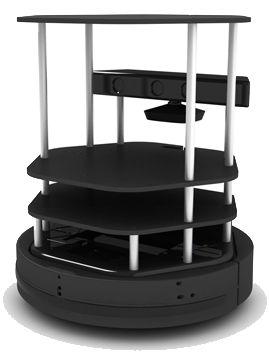
\includegraphics[scale=1.5]{figures/turtlebot.png}
  \caption{Turtlebot robot used in experiments.}
  \label{f:turtlebot_pic}
\end{figure}
